

\documentclass[11pt,a4paper]{article} 

\usepackage[T1]{fontenc}
\usepackage[utf8]{inputenc}
\usepackage{lmodern}
\usepackage[french]{babel}

\usepackage{amsthm}
\usepackage{float}
\usepackage{lmodern}%pour un meilleur rendu des polices
\usepackage{verbatim}%du texte non interprt
\usepackage[cmex10]{amsmath}
\usepackage{amssymb}%maths
\usepackage{xspace}
\usepackage[dvipsnames,svgnames,table]{xcolor}
\usepackage{listings}
\usepackage{fancyhdr}
\usepackage{etoolbox}
\usepackage{titlesec}
\usepackage{titletoc}
\usepackage{lastpage}
\usepackage[bookmarks=true,bookmarksnumbered=true]{hyperref}
\usepackage{ctable} % for \specialrule command
\usepackage{cite}
\usepackage{algorithm2e}
\usepackage{alltt}
\usepackage{array}
\usepackage{mdwmath}
\usepackage{mdwtab}
\usepackage{eqparbox}
\usepackage[caption=false,font=normalsize,labelfont=sf,textfont=sf]{subfig}
\usepackage{dblfloatfix}
\usepackage{url}
\usepackage{tipa}
\usepackage{stmaryrd}

%\usepackage{natbib}
%\usepackage[pdftex]{graphicx}
%\usepackage{framed}
%\usepackage[usenames]{color}

\graphicspath{{img/}}
\DeclareGraphicsExtensions{.pdf,.jpeg,.jpg,.png}

%% taille du papier
\textwidth 16 true cm
\textheight 24 true cm
\addtolength{\hoffset}{-1.5cm}
\addtolength{\voffset}{-1.5cm}

%-------- couleurs
\definecolor{grisf}{rgb}{.47,.47,.47} % barre de droite gris fonce
\newcommand{\colorc}{\color{MidnightBlue}}
\newcommand{\colorb}{\color{NavyBlue}}
\newcommand{\colora}{\color{Cerulean}}

%----------- sections et TOC
% chapitres
\titleformat{\chapter}[display]
  {\normalfont\sffamily\bfseries\huge\colora\centering}{\thechapter}{1ex}
  {{\titlerule[1pt]}\vspace{1.3ex}}[\vspace{1ex}{{\titlerule[1pt]}}]
  
% chapitres etoiles  
\titleformat{name=\chapter,numberless}[display]
  {\normalfont\sffamily\bfseries\LARGE\colora\centering}{}{1ex}
  {{\titlerule[1pt]}\vspace{1.3ex}}[\vspace{1ex}{\titlerule[1pt]}\vspace{2ex}]
  
% sections  
\titleformat{\section}[hang]{\Large\normalfont\sffamily\bfseries\colora}{{\thesection\, }}{0 em}
  {}[{\titlerule[1pt]}\vspace{1ex}]

  
% sous section, sous sous sec, paragraphes  
\titleformat{\subsection}[hang]{\Large\normalfont\sffamily\bfseries\colorc}{{\thesubsection\, }}{0 em}
  {}[{\titlerule}\vspace{.7ex}]
\titleformat{\subsubsection}[hang]{\normalfont\sffamily\bfseries\large}{{\thesubsubsection\, }}{0 em}
  {}[{\color{grisf}\titlerule}\vspace{3pt}]
\titleformat{\paragraph}[runin]{\normalfont\sffamily\bfseries\colorb}{}{0 em}
  {\indent}



%----------------- fancy headers -------------%

\makeatletter
\patchcmd{\@fancyhead}{\rlap}{\color{grisf}\rlap}{}{}
\patchcmd{\headrule}{\hrule}{\color{grisf}\hrule}{}{}
\patchcmd{\@fancyfoot}{\rlap}{\color{grisf}\rlap}{}{}
\patchcmd{\footrule}{\hrule}{\color{grisf}\hrule}{}{}
\makeatother

                                                                    
\fancyhf{}
\fancyhead[R]{\sffamily Rapport HPC/GPGPU }
\fancyfoot[R]{\sffamily\small{\thepage/\pageref{LastPage}}}
\fancyhead[L]{\sffamily\small{Jean-Baptiste Keck}}
\fancyfoot[L]{\sffamily\small{Ensimag -- High Performance Computing -- 2014-2015}}
\renewcommand{\headrulewidth}{0.2pt} %0.4
\renewcommand{\footrulewidth}{0.2pt} %0
\addtolength{\headheight}{0.pt}

\fancypagestyle{plain}{
  \fancyhead{}
  \renewcommand{\headrulewidth}{0pt}
  }
     
  %-- macros --%   
  \def\hlinewd#1{%
      \noalign{\ifnum0=`}\fi\hrule \@height #1 %
  \futurelet\reserved@a\@xhline} 

  
  
  %------------------- front page ------------------%
  \title{
      \bsc{Rapport}
      \vskip 1cm
      {\colorb\textbf{Simulation d'essaims}}
      \vskip 1cm
      {\colorc\textit{High Performance Computing}}
        \vskip 0.1cm
      {\colorc -}
        \vskip 0.3cm
      {\colorc\textit{General-purpose Processing on Graphics Processing Units}}
  }
\author{%
    Jean-Baptiste \bsc{Keck}
    \vskip 0.1cm
    {\huge \bsc{Ensimag -- M2 Msiam}}
    \vskip 1cm
    Gauthier \bsc{Zirnhelt}
    \vskip 0.1cm
    {\huge \bsc{Ensimag}}
}
%\date{27 janvier 2014}
\makeatletter

\def\maketitle{%
    %\thispagestyle{empty}%
    \begin{flushleft}
        \normalfont\LARGE\par
    \end{flushleft}
    \vskip 1cm
    \begin{center}%
        {\colora\specialrule{.2em}{0em}{0em}}
        \vskip 1cm
        {\Huge \@title}%
        \vskip 1cm
        {\colora\specialrule{.2em}{0em}{0em}}
        \vskip 2cm
        {\Huge \@author\par}%
        \vskip 2cm
        {\Huge \@date\par}%
        \vskip 1cm

    \end{center}%
    \clearpage
}


%%%%%%%



\definecolor{lightgray}{gray}{0.9}
\newcommand{\colbox}[1]{\colorbox{lightgray}{$ #1 $}}



\begin{document}
\pagestyle{fancy}

\maketitle

\tableofcontents
\clearpage

\section{Présentation du problème}

\subsection{Étapes de la simulation}
La simulation débute par l'initialisation d'un domaine de taille configurable avec des agents positionnés aléatoirement, aux propriétés également configurables.\\
La boucle de calcul pour la simulation de base est la suivante :
\begin{enumerate}
    \item Calcul des forces appliquées à chaque agent en fonction de tous ceux qui se trouvent à sa portée.
    \item Application des forces précédemment calculées à chaque agent.
    \item Sérialisation des données des agents dans un fichier.
\end{enumerate}
Si un agent sort du domaine pendant un pas de simulation, il est téléporté à l'opposé dans le domaine tout en gardant sa vitesse et sa direction.

\subsection{Coûts des étapes de la simulation}
L'évaluation des forces appliquées à chaque agent est l'opération la plus coûteuse de la simulation, car sa complexité est quadratiquement liée à celle du nombre d'agents à simuler. Les autres étapes n'ont en revanche qu'une complexité directement proportionnelle au nombre d'agents.\\
Nous avons donc dû privilégier l'accélération de l'étape de calcul des forces qui déjà dans le programme de base (640 agents) prenait plus de 99\% du temps de calcul total.



\newpage
\section{Implémentation}

\subsection{Dépendances}
% C++11 MANDATORY [insert perrier référence]
% building the solution = cmake + sm_20 pour cuda à cause de compil séparée
Notre base de code requiert :
\begin{itemize}
    \item Un compilateur supportant le standard C++11 pour la partie CPU.
    \item Une version de nvcc qui compile le standard C++0x minimum pour la partie GPU.
    \item Une carte graphique Nvidia avec l'architecture $sm\_20$ au minimum (pour la compilation et le link séparé des kernels CUDA).
    \item CMake 2.8.12 ou plus (CMake 3.x.x fortement conseillé à cause d'un bug connu dans la compilation des kernels CUDA).
    \item Thrust et Curand pour l'implémentation la plus performante sur GPU.
    \item OpenGL 3.3 ou plus pour les programmes effectuant un rendu 3D.
\end{itemize}


Si vous ne possedez pas de GPU ou si l'architecture CUDA détectée est trop basse, les executables basés sur CUDA ne sont pas compilés.
Il y a donc possibilité de compiler pour CPU seul. L'affichage s'active directement dans le cmake.

Dans le cas où vous n'auriez pas un compilateur supportant C++11, nous fournissons un script qui permet de télécharger et installer GCC 4.8.2 sur votre machine (voir dans la sous-section Scripts utilitaires).\\\\

\subsection{Architecture générale}
% MPI / CUDA merged => mpirun -n 1 ou disable CUDA dans CMakeLists.txt
% les scripts (listés plus bas, pas détailler ici)
% différents éxecutables (sequential / tree???? / main(TODO rename it?) / display)
% différents tests (test_vec : vecteurs<T>           test_messenger : envoi/réception des messages MPI)
% les arbres utilisés
Nous avons opté pour un programme hybride permettant d'utiliser à la fois la performance du calcul distribué avec MPI et également celle du GPGPU avec CUDA. Il est toutefois toujours possible de tester notre programme avec seulement MPI ou seulement CUDA, respectivement en lançant un seul processus ou en désactivant CUDA dans les paramètres au début de $CMakeLists.txt$.\\\\

Les exécutables générés sont les suivants :
\begin{itemize}
    \item $sequential$ : Programme de simulation de base (bruteforce $N^2$ sur CPU, un seul processus)
    \item $main$ : Programme de simulation hybride MPI / CPU / CUDA (bruteforce $N^2$ sur CPU ou GPU)
    \item $display$ : Programme d'affichage des positions des agents simulés 
    \item $tree$ : Programme de démonstration affichant des octtree se faisant remplir.
    \item $cuda$ : Implementation GPU efficace utilisant une grille. Utilise CuRand et Thrust.
    \item $barbecue$ : La même chose que cuda mais avec MPI et un GPU affecté à chaque noeud.
    \item $test\_vec$ : Programme de test des classes de vecteurs
    \item $test\_messenger$ : Programme de test de l'interface de communication construite sur MPI.
\end{itemize}

Nous fournissons en outre gracieusement des scripts utilitaires pour paramétrer l'utilisation de MPI ou de préparer les données à la visualisation.

\subsection{Repartition du code}

Voici la repartition des 13k lignes de code :
    
\begin{figure}[h]
    \begin{center}
            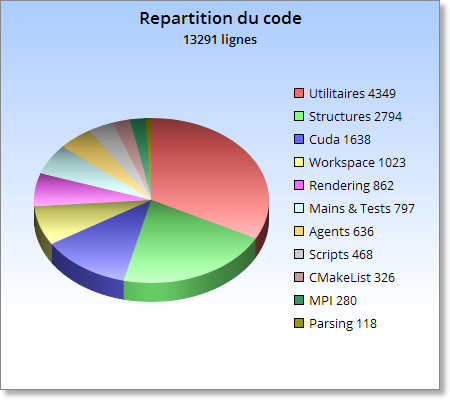
\includegraphics[width=5in]{code} \\
    \end{center}
\end{figure}





\subsection{MPI}
Nous avons opté pour une architecture centralisée pour l'équilibrage de charge . Cette structure peut être un arbre ou une grille classique.
Celle-ci est orchestrée pas le noeud maître, qui envoie des commandes d'initialisation d'agents aux esclaves au tout début de la simulation.
Cette structure, appelée aussi structure globale de simulation, permet de monitorer et distribuer la charge sur tout les noeuds esclaves. Elle situe également spatialement les noeuds esclaves dans le domaine de simulation.
A chaque noeud esclave est affecté un ou plusieurs sous-domaines qui ont eux mêmes leur propre structure de simulation. 
Cette structure locale peut également être un arbre ou une simple grille.

Chaque noeud connait les voisins de ses structures locales ce qui permet un échange de ses agents moyennés localement, ainsi que de trouver à qui envoyer ses agents "sortants". Il envoie aussi périodiquement sa charge d'agents à simuler au processus racine qui peut prendre la décision de rééquilibrer l'affectation des domaines aux processus.

\subsection{CUDA}

Il y a deux implémentation Cuda. L'une plus brute, ne fait qu'un bruteforce sauvage de la simulation en $N^2$ mais en profitant de la douceur des coeurs d'une carte graphique.
L'autre plus élégante permet de simuler les agents sur une structure acceleratrice afin de passer en $n^2$ local avec $n << N$. Voici un appercu rapide de l'algorithme sans initialisation :

\vskip 0.5cm

\begin{algorithm}[H]
    \KwData{Agents^t (position + vitesses + forces)}
    \KwResult{Agents^{t+1}}

    \While{Simulation not ended}{
        ComputeCellId$<<<>>>$()     //kernel to compute id of the boid in the local structure\;

        Sort boids in place according to computed cell id.

        Find non empty cell ids with conditional reduction.

        Find filled cells agent count with conditional reduction.

        Deduce offsets in the boid array with prefix sum.

        Generate an array that contains cell status (either filled or not), usefull for neighbors lookup

        ComputeMeanagent$<<<>>>$ //Compute per non empty cell mean position and mean velocity

        ComputeForces$<<>>>$() //Compute internal and external forces and store it in temporary array

        IntegrateScheme$<<<>>>$() //Simple Euler integration
    }
    \caption{Algorithme élégant}
\end{algorithm}

\vskip 1cm
Toute les réductions et sommes cumulatives sont réalisées avec la librairie $Thrust$.
L'initialisation est réalisée avec la librairie $CuRand$. Ceci permet d'initialiser confortablement 250 millions d'agents (position + vitesse) en moins d'une seconde sur deux GTX670 4Go.

\begin{figure}[h]
    \begin{center}
            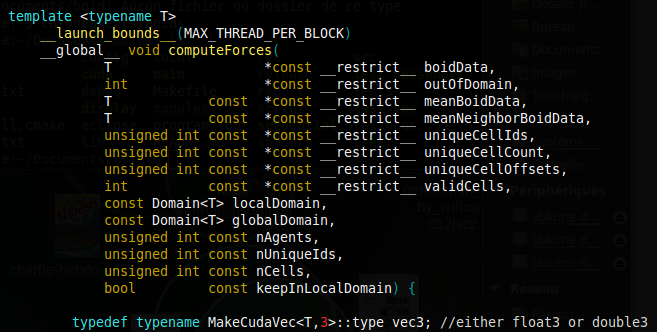
\includegraphics[width=6in]{kernel} \\
            \caption{Petit kernel}
    \end{center}
\end{figure}

\vskip 0.2cm
Nous utilisons également un seul bloc de mémoire coalescente pour les gents. Pour plus d'information voir dans $src/boids/$ les sources [const]vectorMemoryView.hpp thrustVectorMemoryView.hpp, [const]boidMemoryView.hpp, thrustBoidMemoryView.hpp.

\subsection{CUDA-MPI}

L'algorithme précédent à été adapté pour MPI. A chaque noeud (rank), on affecte un GPU sur la machine (le rank modulo le nombre de GPUs). 
L'initialisation a été adaptée pour ne se faire que sur un seul GPU. Quelle fut notre tristesse quand nous apprîmes que Thrust ne gérait apparemment pas la mémoire de plusieurs GPUs (nous en sommes pas sures par manque de documentation disponible, mais après moultes essais cela semble être effectivement le cas). Nous n'avions malheuresement plus le temps de wrapper les vecteurs Thrust avec notre gestionnaire de mémoire maison (voir $src/cuda/memoryManager/$).


\subsection{Structures}
\subsubsection{Grilles}
    
    Structure de grille basé sur le rayon d'effect maximum des forces. 
    Voir $src/struct/grid$.

\subsubsection{Arbres}
    
    Structure d'arbre de type octtree ou kd-tree. 
    Voir $src/struct/tree$.

    Petite appercu des arbres avec l'executable $tree$ :

    \begin{figure}[h]
    \begin{center}$
        \begin{array}{ccc}
            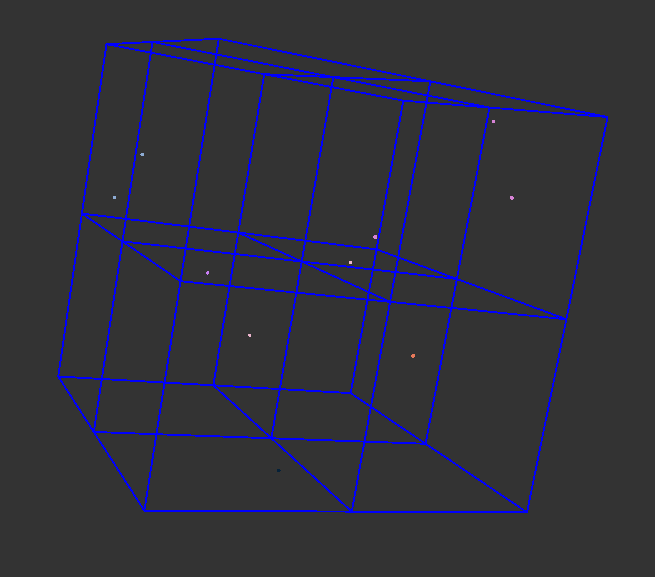
\includegraphics[width=1.75in, height=1.75in]{tree_1} &
            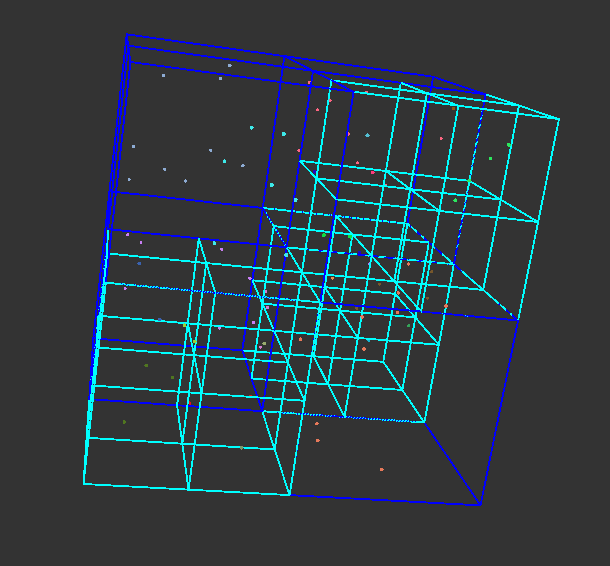
\includegraphics[width=1.75in, height=1.75in]{tree_2} &
            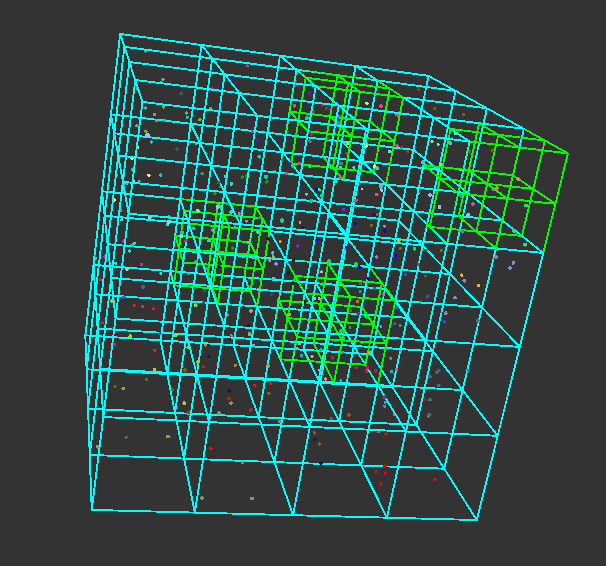
\includegraphics[width=1.75in, height=1.75in]{tree_4} \\
            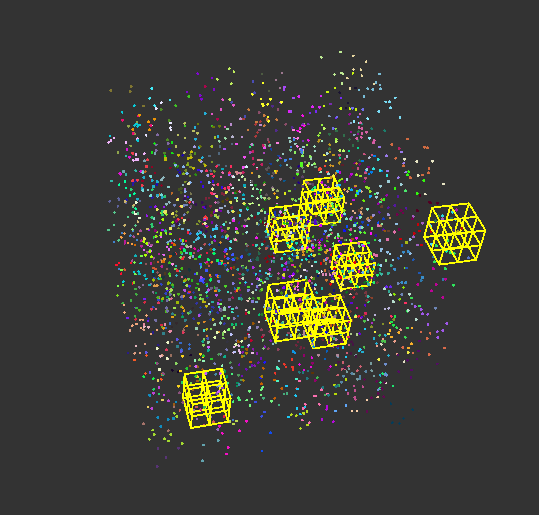
\includegraphics[width=1.75in, height=1.75in]{tree_5} &
            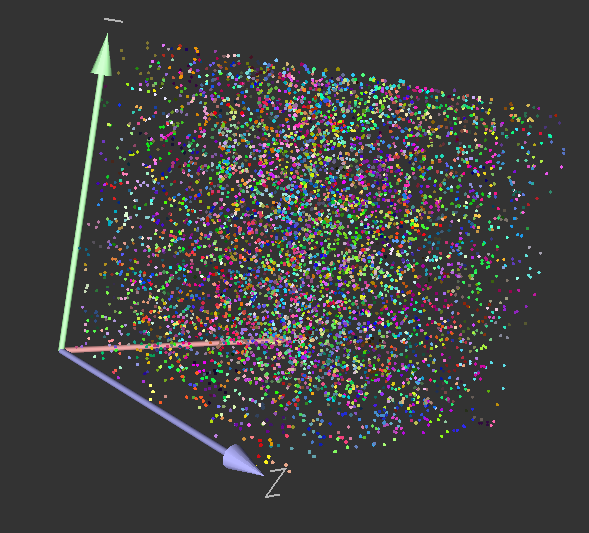
\includegraphics[width=1.75in, height=1.75in]{tree_6} &
            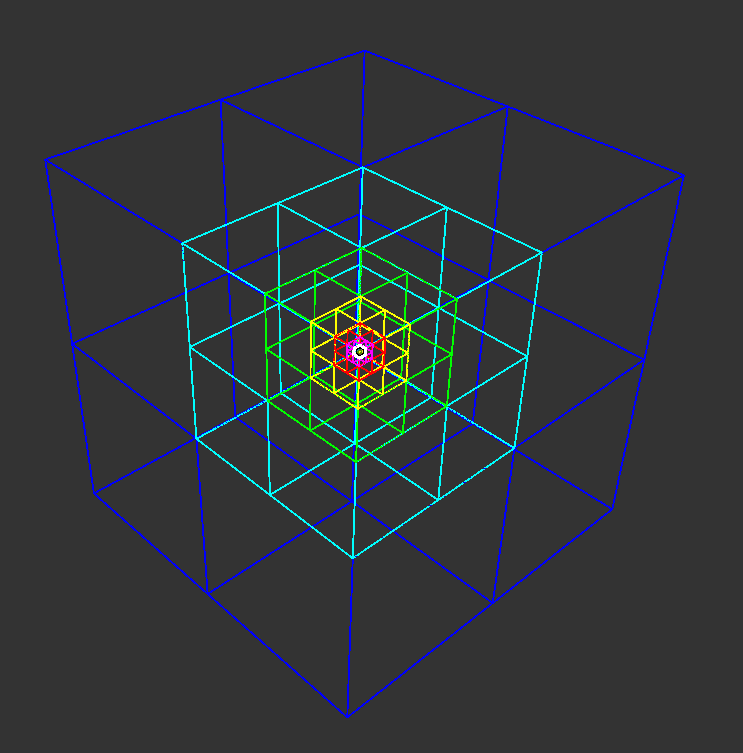
\includegraphics[width=1.75in, height=1.75in]{tree_10} \\
            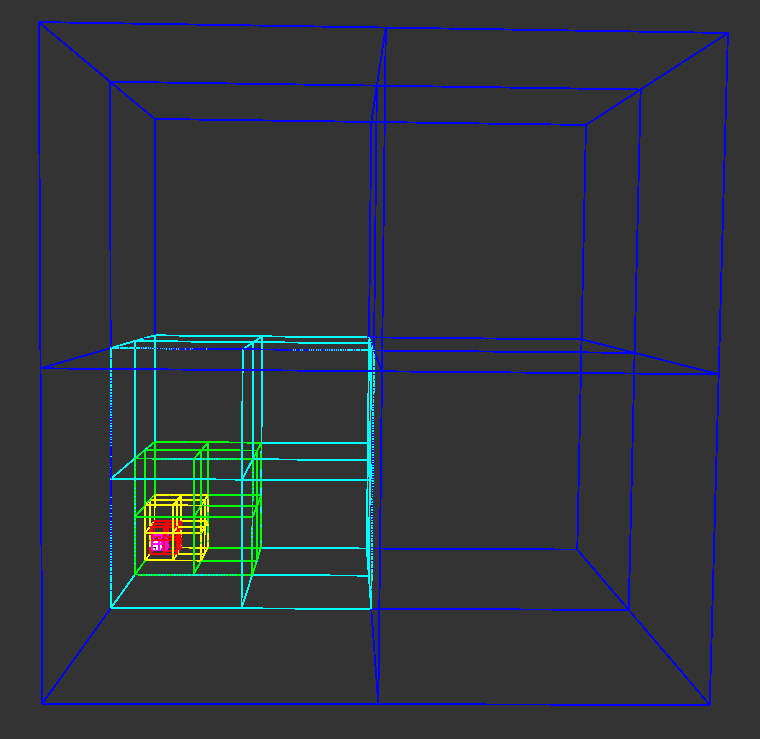
\includegraphics[width=1.75in, height=1.75in]{tree_7} &
            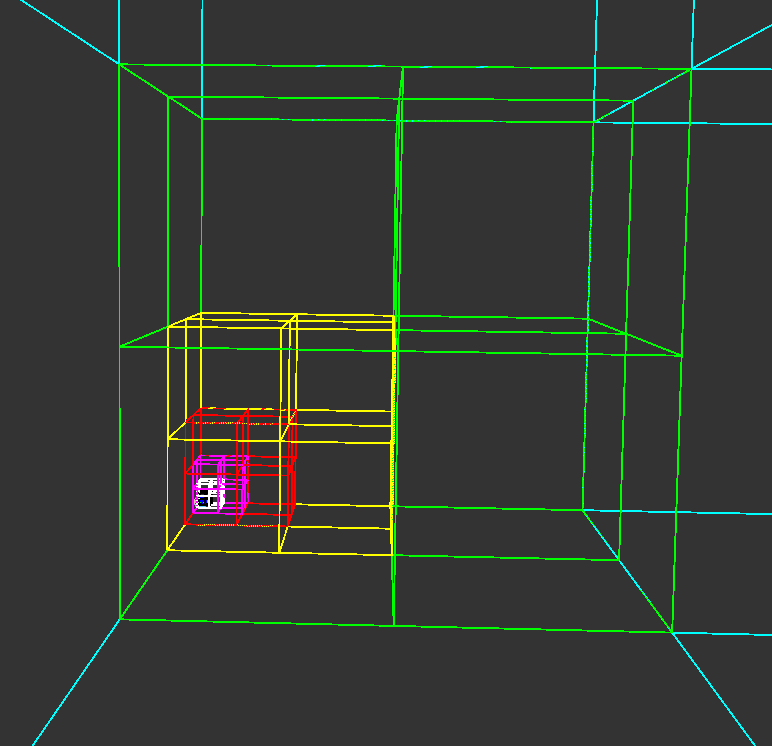
\includegraphics[width=1.75in, height=1.75in]{tree_8} &
            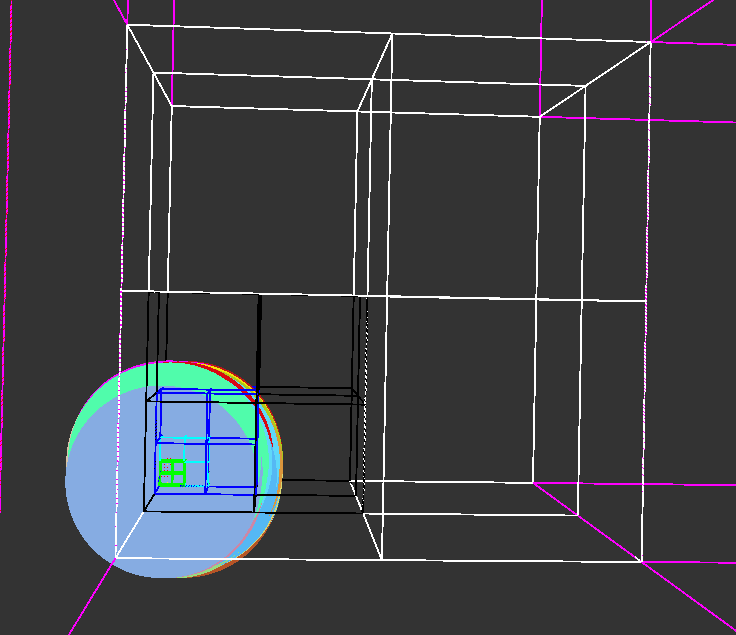
\includegraphics[width=1.75in, height=1.75in]{tree_9} \\
        \end{array}$
    \end{center}
\end{figure}

\subsection{Scripts utilitaires}
% Donner leur fonction
Les scripts utilitaires fournis avec nos sources sont les suivants :
\begin{itemize}
    \item $dependancies.sh$ : Installe les dépendances de GCC 4.8.2 
    \item $gcc.sh$          : Installe GCC 4.8.2 (pour le support de C++11)
    \item $genAppFile.sh$   : Génère un fichier Appfile automatiquement à partir d'une liste d'host en stdin.
    \item $merge\_files.py$ : Fusionne tous les fichiers de données issus de la simulation par des processus différents en un seul fichier.
    \item $path.sh$         : Corrige le $.bashrc$ des ensipc.
    \item $scanner.sh$      : Établit rapidement la liste des machines (ensipc) en ligne.
    \item $utils.sh$        : Contient des fonctions utilitaires utilisées par $gcc.sh$.
    \item $visu.sh$         : Script permettant de visualiser les résultats avec $gnuplot$ sur une machine ne permettant pas de compiler et/ou eexécuter le programme de visualisation d'agents fourni.
\end{itemize}


\subsection{Visualisation}
% Expliquer comment marche le viewer (merge fichiers, parsing fichier, sprites)
Nous fournissons un programme permettant de visualiser les agents simulés dans de meilleures conditions qu'avec gnuplot.
Celui-ci se lance avec la commande $./display$ et va par défaut lire le fichier résultant de l'opération de fusion réalisée par le script $merge\_files.py$. Il est possible de modifier le fichier lu par défaut en en spécifiant un autre à l'aide de l'option $-f$ du programme.\\

Le progamme affiche chaque agent sous la forme d'une sprite faisant face à la caméra. Cette sprite contient un cercle coloré représentant le type d'agent affiché. Cette technique de rendu très simple permet d'afficher beaucoup plus d'agents simultanément que si l'on représentait chaque agent par un volume texturé par exemple, ce qui permet de conserver une visualisation fluide pour grand nombre d'agents.\\

L'étape de la simulation en cours de visualisation est affichée en bas à gauche de l'écran. 
La lecture est pausable avec la touche $entr\acute{e}e$. 
Il est possible de rembobiner la simulation au démarrage en appuyant sur la touche $r$.
Les axes (utilisés pour avoir un repère fixe) sont affichables en utilisant la touche $a$.



\section{Résultats}
% En gros, surtout des images commentées

\subsection{CPU bruteforce}
\subsection{GPU bruteforce}
\subsection{GPU efficace}

\begin{figure}[H]
    \begin{center}$
        \begin{array}{cc}
            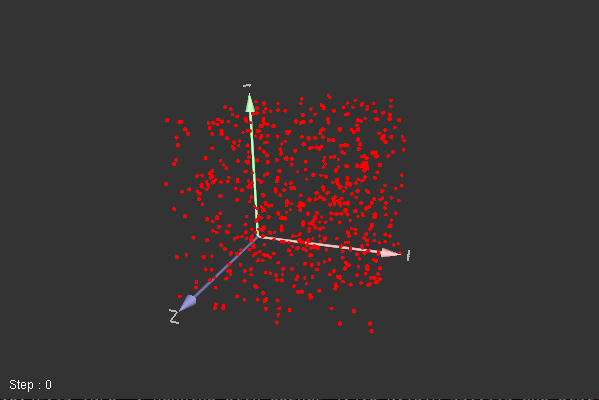
\includegraphics[width=3in, height=2in]{img/visu0.png} &
            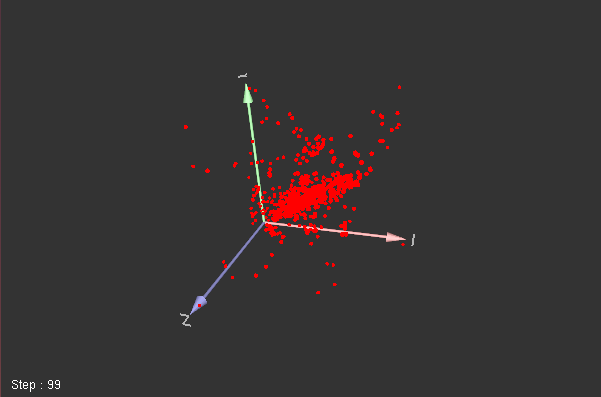
\includegraphics[width=3in, height=2in]{img/visu.png}
        \end{array}$
        \caption{Début d'une simulation avec des agents aux positions, vitesses, et directions aléatoires à gauche et visualisation d'un essaim de particules formé durant la simulation à droite.}
    \end{center}
\end{figure}



\subsection{Performances}
% Tableau comparatif : méthode(sequential, mpi seul, cuda seul, hybride) / nombre de boids (100-1000-10k-1M-...) [/ nombre de process / gpu]
% Peut-être aussi en fonction des rayons?

\subsection{Qualité de la simulation}
% Vite dit, visuellement dans le viewer
% formation d'esseims avec la force de cohésion : ok
% force de séparation => esseims assez étalés : ok
% alignement dans un direction commune qui sera conservée sauf collisions : ok 
Nous avons fait des essais de simulation en modifiant les paramètres de la simulation et observé un comportement cohérent des agents lorsqu'une force était prépondérante sur les autres.
\begin{itemize}
    \item La force de cohésion permet la création d'essaims d'agents.
    \item La force de séparation sépare les agents afin de ne pas avoir d'essaims d'une densité trop élevée, mais peut aussi rendre impossible la formation de ces essaims si elle est trop grande.
    \item La force d'alignement force les agents à tous aller dans la même direction, ce qui permet globalement de conserver un essaim dans le temps tant qu'il n'entre pas en collision avec un autre.
\end{itemize}



\section{Perspectives d'amélioration}

\subsection{Tolérance à la faute pour MPI}
% timeout sur les messages MPI au lieu de bloquer indéfiniment.
Nous utilisons des messages MPI bloquants en réception, ce qui fait que notre système ne tolère aucune perte de message. Normalement, aucun message n'est perdu par MPI, mais dans le cas où une machine subit une défaillance, tout notre système se trouvera bloqué et il faudra recommencer la simulation.\\
Une amélioration consisterait ici à implanter un système tolérant à la faute en utilisant un système de timeout pour détecter les fautes, ainsi qu'un système de réplication des données des agents entre les différentes machines pour réaffecter les tâches de calcul.

\subsection{Visualisation de la simulation}
Nous aurions aimé avoir le temps nécessaire à l'amélioration de notre programme de visualisation. Les améliorations envisagées sont les suivantes :
\begin{itemize}
    \item Affichage à l'aide d'un triangle orienté de la direction d'un agent
    \item Sélection du numéro de l'étape à visualiser pendant le mode pause
\end{itemize}

\subsection{Différents types d'agents}
Nous avons réfléchi à l'ajout de surfaces non traversables par les agents normaux à base d'un type d'agent à position fixée dont l'unique rôle aurait été de repousser les autres agents.\\
Nous avons également pensé ajouter des agents prédateurs qui produiraient une force de répulsion importante à l'encontre des autres agents qui seraient ses proies.


\section{Conclusion}

Nous n'avons pas pu implémenter tout ce que nous avions prévu, ni assembler toutes les briques de nos programmes. 
Les diverses implémentation proposées performent plus ou moins efficacement sur le problème de la simulation d'essaim.
\vskip 0.2cm
Sans même avoir des kernels super optimisés, les GPU offrent des performances toujours bluffantes quand l'algorithme le permet et quand les structures sont adapatés au modèle SIMD comme c'est le cas ici.
\vskip 0.2cm
A cause de la lattence réseau (100Mbps), l'implémentation efficace en GPU locale exécuté un GPU correct est certainement plus efficace que tout les GPUs de l'Ensimag réunnis. Nous n'avons malheuresement pas pu effectuer une simulation de cette échelle à l'Ensimag car c'est tout simplement impossible.
\vskip 0.2cm
Grosse deception du coté de MPI qui ne semble pas pouvoir gérer la mémoire paginée et surtout pour Thrust qui ne semble pas gérer la mémoire sur plusieurs cartes graphiques. Des problemes mémoires, encore présents dans le rendu, sont tout simplement impossible à déboguer car l'execution de cuda-gdb, cuda-memcheck ou encore nsight sur les cas de faute mémoire génère un deadlock de driver nvidia (340.65) qui se bloque dans un mutex dans la libcuda... La seule solution restante étant de redémarer le système pour reinitialiser les GPUs.
\vskip 0.2cm
Il faudrait clairement commencer le projet plus tôt dans l'année. En plus de posséder des librairies et compilateurs du néendertal, les architectures de l'école sont bien sont trop héréroclites et avec une période de fonctionnement aléatoire ce qui rend la tache très complexe. On rapellera la disparition soudaine et tragique du cuda toolkit 6.5 qui a marqué tous les esprits en ce début d'année alors qu'elle permettait le support experimental du C++11 ! De plus le nouveau serveur de cette année (pcserveur) ne permet plus que d'utiliser 2 coeurs virtuels (depuis le projet GL), ce qui est une régression énorme depuis l'age d'or de telesun et ses 48 coeurs accessibles à tout Ensimag lambda en ssh (et sans VPN) qui faisait tourner fièrement nos programmes multithreadés en ADA83. 

\end{document}
